\documentclass[10pt,conference,letterpaper]{IEEEtran}

\usepackage{cite}
\usepackage{amsmath,amssymb}
\usepackage{graphicx}
\usepackage{textcomp}
\usepackage{booktabs}
\usepackage{multirow}
\usepackage{url}

\def\BibTeX{{\rm B\kern-.05em{\sc i\kern-.025em b}\kern-.08em
    T\kern-.1667em\lower.7ex\hbox{E}\kern-.125emX}}

\begin{document}

\title{Data-Oriented Design for MSCKF Visual-Inertial Odometry:\\
A Cache-Layout Reimplementation with Measured Parity to OpenVINS}

\author{
\IEEEauthorblockN{Shafwan Safi, Nikhil Vashisht, Pranjal Upadhyay}
\IEEEauthorblockA{Indian Institute of Science Education and Research (IISER) Bhopal}
}

\maketitle

\begin{abstract}
We present a data-oriented C++ reimplementation of the multi-state constraint
Kalman filter (MSCKF) visual-inertial odometry (VIO) pipeline used by
OpenVINS, built around fixed-capacity, allocation-free per-frame state and a
feature database that separates search keys from payloads. Benchmarked
against official OpenVINS through the identical rosbag transport on ten
public sequences (EuRoC MH/V1, KAIST circle/infinity), the reimplementation
matches OpenVINS's absolute trajectory error (ATE) to within measurement
parity --- better on 4 of 10 sequences, mean ATE 0.156\,m versus 0.158\,m,
geometric-mean ratio 1.06 --- while running end-to-end at 1.76--2.10$\times$
the wall-clock throughput (\texttt{hyperfine}, warmed cache, 5 runs), and
converging with zero re-tuning on an independent third dataset family (TUM
VI, fisheye, mean ATE 0.062\,m across its six room sequences at parity with
OpenVINS). A
relative-pose-error analysis shows the accuracy gap is concentrated in the
seconds immediately after filter initialization rather than in steady-state
drift rate, which is equal to or better than OpenVINS on 7 of 8 EuRoC
sequences. Per-frame latency analysis sharpens the throughput claim: at the
99th percentile the reimplementation's frame latency advantage
(1.75--2.05$\times$) exceeds its mean advantage, and OpenVINS's worst frame
on one sequence exceeds its own frame deadline. Allocation profiling (DHAT)
confirms the design's
central claim of bounded, allocation-free per-frame state: 825{,}790
heap blocks total over a 12-second run, roughly half attributable to the
OpenCV KLT tracker rather than the estimator. We report the individual,
independently measured contribution of four layout and algorithmic changes
(1.34$\times$ combined, every trajectory bit-identical before and after), an
embedded validation of both estimators on all ten sequences on an NVIDIA
Jetson Orin Nano under the identical toolchain container, where the
advantage transfers in direction but narrows (1.16--1.61$\times$ median
per-frame latency, bounded 184--199\,MB peak memory), a cross-platform
floating-point defect found and fixed during that deployment, and the scope
of what remains unvalidated. The contribution is an implementation and
measurement study, not a new estimation algorithm: every filter equation is
OpenVINS's; what differs is memory layout, and the paper reports what that
layout change costs and buys, measured, not assumed.
\end{abstract}

\begin{IEEEkeywords}
visual-inertial odometry, MSCKF, data-oriented design, embedded robotics, cache-efficient state estimation
\end{IEEEkeywords}

\section{Introduction}

Visual-inertial odometry (VIO) is a per-frame, real-time estimation problem:
every camera frame must be processed within its exposure interval or the
system falls behind the sensor stream it is trying to track. OpenVINS
\cite{geneva2020openvins} is a widely used, carefully engineered open-source
MSCKF \cite{mourikis2007msckf} implementation and is the accuracy and design
reference for this work. Its C++ implementation follows conventional
object-oriented design: polymorphic state variable types, \texttt{std::vector}
containers, and heap-allocated per-feature and per-measurement objects.

This is not a criticism of OpenVINS's engineering; it is an observation about
what that design pattern costs on a per-frame hot path, independent of the
estimator's mathematics. Mike Acton and Richard Fabian's data-oriented design
(DOD) literature \cite{fabian2018dod} argues that on such paths, the layout of
data in memory --- not the algorithm expressed over it --- is usually the
dominant cost, and that object-oriented abstractions frequently hide layout
decisions a profiler would reject. This paper tests that argument on a
production-shaped VIO pipeline rather than a microbenchmark: we reimplement
OpenVINS's MSCKF pipeline in C++ under a small set of house rules --- no
per-frame heap allocation, no virtual dispatch, all state in fixed-capacity
tables, one transform per table --- and measure the result against the
original on identical data through an identical transport.

The result is not a strict win. Reporting it as one would misrepresent the
data: the reimplementation is faster by a wide, consistent margin, and it is
accuracy-competitive but not accuracy-superior. Section~\ref{sec:results}
presents both findings without rounding the second one away, and
Section~\ref{sec:limitations} states plainly what has not yet been validated,
including the parts of the embedded comparison that remain unmeasured
(thermals, frequency state, wall-clock).

\textbf{Contributions.}
\begin{itemize}
\item A cache-layout redesign of the OpenVINS MSCKF pipeline validated
  bit-identical against the original estimator's mathematics across ten
  trajectories, with per-optimization, independently measured speedups
  (Table~\ref{tab:ablation}).
\item A same-transport benchmarking methodology (identical bag, identical
  transport, both estimators as ROS nodes in the identical toolchain
  container) plus a measured decomposition of the two environmental
  confounds: transport choice moves the ATE by 0--5.2\% across the EuRoC MH
  sequences, while toolchain choice moves it by up to 23\% on identical
  code and data --- an ATE quoted without both cannot be reproduced.
\item A relative-pose-error decomposition showing that an aggregate ATE
  comparison can hide a steady-state accuracy advantage behind an
  initialization-timing artifact, and a worked example (Section~\ref{sec:rpe})
  where exactly this happens.
\item A reported, not silently avoided, cross-platform numerical defect
  (Section~\ref{sec:embedded}): a companion-matrix eigenvalue convergence
  gate tuned implicitly for x86-SSE2 rounding that rejected a correct solution
  under ARM-NEON rounding, found via a Jetson Orin Nano deployment,
  root-caused, and fixed with the fix verified not to move any of
  the ten trajectories on x86.
\item An embedded validation of the same comparison on the Jetson Orin Nano
  Super: both estimators, all ten sequences, per-frame latency and peak RSS
  under the identical toolchain container as x86
  (Section~\ref{sec:embedded}), including the finding that the desktop tail
  advantage does \emph{not} grow on the small core.
\end{itemize}

\section{Related Work}

\textbf{OpenVINS} \cite{geneva2020openvins} is the reference implementation
and accuracy baseline throughout this paper; every comparison in
Section~\ref{sec:results} is against an unmodified, independently rebuilt
copy of it, run through the same transport as the reimplementation under
test.

\textbf{SchurVINS} \cite{fan2024schurvins} restructures the MSCKF update to
exploit the block-diagonal structure of the per-measurement Hessian, reducing
an update from $O(m^3)$ to linear in the number of features by eliminating
the landmark block once per feature via a Schur complement before the pose
update. We reimplemented SchurVINS's update in the same data-oriented layout
(fixed-capacity buffers, no per-frame allocation) as an alternate MSCKF
update path, gated behind a runtime flag and \emph{off by default}; every
benchmark number in this paper uses the primary MSCKF/SLAM update path, not
the SchurVINS path.

\textbf{sqrtVINS} \cite{peng2025sqrtvins} contributes two ideas this
pipeline uses directly and attributes precisely: a square-root-form EKF
update that factors rather than inverts the innovation covariance
(Section~\ref{sec:sqrtform}), and a feature-less dynamic initializer
(Section~\ref{sec:featureless-init}) that recovers velocity and gravity from
bearing-only epipolar geometry without ever triangulating a 3D point, which
this pipeline uses as its primary EuRoC initialization path.

\textbf{The hovering classifier} follows Kottas, Wu, and Roumeliotis
\cite{kottas2013hover}: a rotation-compensated bearing-vector residual
between consecutive clones, with hysteresis, used here to switch clone
marginalization between FIFO (generic motion) and LIFO (hovering) so a
stationary interval does not squeeze a genuine-motion baseline out of the
sliding window.

\section{System Design}

\subsection{The house rules}
\label{sec:rules}

The reimplementation follows a small, fixed set of constraints applied
uniformly to every file on the per-frame path:

\begin{enumerate}
\item \textbf{No per-frame allocation.} No \texttt{new}, no
  \texttt{std::vector::push\_back}, no \texttt{std::string}, no
  \texttt{std::function}. All per-frame state lives in fixed-capacity structs
  or a bump-pointer arena reset at a known frame boundary.
\item \textbf{All memory bounded at initialization.} Every array carries a
  compile-time capacity constant; \texttt{init\_*()} functions validate the
  configured maximum against it and abort loudly rather than corrupt memory
  silently at the first overflow.
\item \textbf{No virtual dispatch, no inheritance, no RTTI on the hot path.}
  Behavior that varies by case varies by which fixed-layout table a row
  belongs to and which transform runs over that table, decided once per
  frame outside the inner loop, not per-row inside it.
\item \textbf{Existence-based processing.} Table membership is the boolean.
  A feature eligible for triangulation is one already present in a
  pre-filtered pointer array built once upstream; the triangulation loop
  itself carries no per-row conditional.
\item \textbf{Transforms are pure over their row.} A transform reads its
  inputs and writes its outputs once; it does not read back what it just
  wrote, so aliasing analysis and the accuracy argument for a given change
  both stay tractable.
\end{enumerate}

These are restatements of data-oriented design as documented by Fabian
\cite{fabian2018dod}; the contribution here is applying them uniformly to a
full, non-trivial MSCKF pipeline and measuring the result, not the rules
themselves.

\subsection{The feature database}

The most consequential single layout decision is in the feature database.
OpenVINS's \texttt{FeatureDatabase} is a hash map from feature ID to a
heap-allocated feature object; the reimplementation uses a fixed array of
2048 feature slots (measured peak occupancy across all ten benchmark
sequences: 250, on MH\_04) with search order and payload storage
\emph{physically separated}: an \texttt{order[]} array of 4-byte slot indices
is kept sorted by feature ID, while the 2400-byte feature payloads
themselves never move once written. Before this change, the database kept
payloads physically sorted by ID, so every newly observed feature required a
\texttt{memmove} of the array tail to preserve order --- measured at 9{,}556
feature copies per frame, 22.9\,MB/s of pure \texttt{memcpy}, to maintain an
ordering over what is structurally a 4-byte key. Separating key from payload
turns that insertion cost into a shift of 4-byte integers instead of
2400-byte structs, with feature payload addresses now stable across a
compaction (freed slots are recycled through a stack rather than by
shifting), which is strictly safer for any caller that had cached a pointer
across a cleanup pass.

\subsection{Square-root-form EKF update}
\label{sec:sqrtform}

The EKF update is restructured following sqrtVINS's \cite{peng2025sqrtvins}
central principle --- never invert what can be factored. With innovation
covariance $S = H_{\text{stack}} P H_{\text{stack}}^\top + R$, the
conventional form computes $S^{-1}$ explicitly (an $m^3$ solve against the
identity) and then $K = M_a S^{-1}$ as a separate dense product. Writing
$S = LL^\top$ (Cholesky) and $G := M_a L^{-\top}$:
\begin{equation}
K M_a^\top = M_a S^{-1} M_a^\top = (M_a L^{-\top})(M_a L^{-\top})^\top = GG^\top
\end{equation}
so the explicit inverse and the separate $K$ product both disappear, and the
covariance update becomes a symmetric rank-$k$ update on the upper triangle
of $P$. This is not only faster: it also eliminates a real correctness
defect present in an earlier, dense form of this update. $K M_a^\top$ is
symmetric in exact arithmetic but not in floating point, and collapsing the
update to the dense form \texttt{Cov -= K * M\_a.transpose()} allows that
asymmetry to drive covariance diagonals negative within a few hundred
frames --- measured to abort the filter on EuRoC MH\_01 at approximately
$t{=}16$\,s. The rank-$k$ form is symmetric by construction and does not
exhibit this failure.

For scale: the speed contribution of this change is real but small ---
0.29\,ms per frame across the two affected stages (Table~\ref{tab:ablation},
row 3), roughly 8\% of the total per-frame reduction from all accepted
changes. The bulk of the end-to-end speedup comes from the memory-layout
decisions, not from this algorithmic restructure; the square-root form's
primary contribution is the correctness property above, with the speed
difference a secondary effect.

\subsection{Feature-less dynamic initialization}
\label{sec:featureless-init}

The standard MSCKF dynamic initializer solves jointly for feature depths,
velocity, and gravity from a short window of vision and IMU preintegration.
Over a short, low-parallax window this system is close to rank-deficient in
the feature block: measured against Leica ground truth on EuRoC MH\_02, it
recovered a velocity of 0.162\,m/s where ground truth was 0.029\,m/s, and the
resulting run diverged, while every quality metric available to the filter
at initialization time --- residual, conditioning, recovered gravity
direction --- looked healthy. Following sqrtVINS Sec.~V-A
\cite{peng2025sqrtvins}, the pipeline's primary EuRoC initializer instead
recovers velocity and gravity \emph{without} ever estimating a 3D point:
bearings from a feature observed in two frames, rotated into a common
reference frame, span an epipolar plane whose normal is perpendicular to the
relative translation direction; stacking this constraint over many features
and combining it with IMU preintegration (which supplies the translation
\emph{with} scale) yields a linear system in velocity and gravity alone. This
initializer fires successfully at the minimum admissible window
(3 feature pairs, 3 time instants) on all eight EuRoC sequences benchmarked
in this paper.

\section{Experimental Setup}
\label{sec:setup}

\subsection{Hardware}
All x86 measurements were taken on an AMD Ryzen~9 7950X (16 cores / 32
threads), 61\,GB RAM, running the estimator and OpenVINS as ROS~1 Noetic
nodes inside an identical Docker container on both sides of every comparison.

\subsection{Same-transport methodology}
Every accuracy and wall-clock comparison in this paper runs both estimators
as ROS~1 nodes consuming the identical rosbag through the identical
transport, rather than comparing a reimplementation's native dataset reader
against the reference implementation's ROS node. We measured what transport
choice alone is worth: running the reimplementation on all five EuRoC MH
sequences through the dataset's raw ASL folder format versus through a
played rosbag, inside the identical toolchain container, moves the ATE by
0--5.2\% per sequence (e.g.\ MH\_01 0.1293\,m through both transports;
MH\_02 0.2080\,m ASL versus 0.1978\,m bag). A previously reported
approximately 15\% transport effect was a misattribution: its ASL-side
figure (0.1131\,m) could not be reproduced at any commit we tested
(Section~\ref{sec:toolchain}), and the large environmental effect on
accuracy is the \emph{toolchain}, not the transport. The V1 sequences are
quoted from the ASL transport only, because their bag ground-truth topic
requires a conversion the bag runner does not implement; MH and KAIST bag
transport carries ground truth directly.

\subsection{Toolchain confound}
\label{sec:toolchain}
Transport is not the only environmental variable an ATE figure silently
carries. Building the identical estimator code from the identical commit
against identical data, differing only in the toolchain (OpenCV 4.2.0 with
g++ 9.4.0 in a pinned Docker container versus OpenCV 4.5.4 with g++ 11.4.0
on the host), reproduces most EuRoC sequences within about 1\% but differs
by 23\% on MH\_02 and 8\% on V1\_01 (Table~\ref{tab:toolchain}). The
frontend is OpenCV's KLT tracker, so the library version is part of the
reported result, and the divergence concentrates exactly where reviewers
spot-check. We quote an environment with every ATE in this paper; an ATE
quoted without its transport and toolchain cannot be reproduced.

\begin{table}[t]
\caption{Identical code and data, two toolchains (ATE RMSE, m;
$\Delta$ relative to the container figure). Most
sequences agree within a few percent; MH\_02 differs by 23\%.}
\label{tab:toolchain}
\centering
\begin{tabular}{lrrr}
\toprule
Sequence & container & host & $\Delta$ \\
\midrule
MH\_01 & 0.1293 & 0.1282 & 1\% \\
MH\_02 & 0.2080 & 0.1595 & 23\% \\
MH\_03 & 0.2343 & 0.2234 & 5\% \\
MH\_04 & 0.4267 & 0.4416 & 3\% \\
MH\_05 & 0.3285 & 0.3115 & 5\% \\
V1\_01 & 0.0545 & 0.0499 & 8\% \\
V1\_02 & 0.0482 & 0.0553 & 15\% \\
V1\_03 & 0.0550 & 0.0564 & 3\% \\
\bottomrule
\end{tabular}
\end{table}

\subsection{Datasets}
Ten public sequences: EuRoC MH\_01--MH\_05 (machine hall) and V1\_01--V1\_03
(vicon room), and two KAIST Complex Urban sequences (circle, infinity),
covering handheld/UAV indoor flight and ground-vehicle outdoor driving.
Ground truth for MH\_* comes from the bag's \texttt{/leica/position} topic;
V1\_* publishes vicon pose on a differently named topic
(\texttt{/vicon/firefly\_sbx/firefly\_sbx}, a \texttt{TransformStamped})
which required a small conversion script, since the estimator's default
ground-truth extraction assumed the \texttt{/leica/position} topic name and
silently produced an empty reference file on V1\_* until this was found and
fixed.

\subsection{Wall-clock methodology}
Wall-clock comparisons use \texttt{hyperfine} 1.18.0, \texttt{-i} (ignore
non-zero exit --- OpenVINS's ROS node throws a benign
\texttt{class\_loader::LibraryUnloadException} at shutdown, after all
estimation work and file output are complete), one warmup run, five
measured runs.

\subsection{Allocation methodology}
Allocation profiling uses \texttt{valgrind}'s DHAT tool over 12 seconds of
EuRoC MH\_01 played through the ASL runner, ranked both by allocation count
and by total bytes, since the two rankings identify different defects: a
site making many small allocations and a site making few very large ones are
both invisible to the other's ranking.

\section{Results}
\label{sec:results}

\subsection{Accuracy}

\begin{table}[t]
\caption{Absolute Trajectory Error (ATE RMSE, metres), same rosbag transport
for both estimators. Both columns re-measured on 2026-08-30 from the current
tree inside the pinned toolchain container; every figure in this table is
reproducible from the released artifact.}
\label{tab:ate}
\centering
\begin{tabular}{lrrr}
\toprule
Sequence & Ours & OpenVINS & Ratio \\
\midrule
MH\_01\_easy      & 0.1293 & \textbf{0.1180} & 1.10 \\
MH\_02\_easy      & 0.1978 & \textbf{0.1616} & 1.22 \\
MH\_03\_medium    & \textbf{0.2342} & 0.2486 & 0.94 \\
MH\_04\_difficult & 0.4267 & \textbf{0.4110} & 1.04 \\
MH\_05\_difficult & \textbf{0.3163} & 0.3195 & 0.99 \\
V1\_01\_easy      & 0.0751 & \textbf{0.0634} & 1.18 \\
V1\_02\_medium    & 0.0589 & \textbf{0.0573} & 1.03 \\
V1\_03\_difficult & \textbf{0.0550} & 0.0595 & 0.92 \\
KAIST circle      & 0.0374 & \textbf{0.0305} & 1.23 \\
KAIST infinity    & \textbf{0.0261} & 0.0284 & 0.92 \\
\midrule
Mean              & 0.1557 & 0.1583 & --- \\
Geometric mean of ratio & \multicolumn{2}{c}{} & 1.056 \\
\bottomrule
\end{tabular}
\end{table}

Table~\ref{tab:ate} shows the reimplementation better on 4 of 10 sequences,
worse on 6, mean ATE 0.1557\,m against OpenVINS's 0.1583\,m, geometric-mean
per-sequence ratio 1.056. We report this as \emph{accuracy parity}, not an
accuracy advantage. Every figure in the table was re-measured for this paper
from the current code in the pinned container (both estimators), with
OpenVINS's ground-truth-adjacent outputs produced by its own state recorder;
the V1 rows are evaluated against the dataset's ASL ground-truth stream for
both estimators because the bag transport does not carry that topic in a
form the extraction handles.

\begin{figure*}[t]
\centering

\includegraphics[width=\textwidth]{figs/all_sequences.png}
\caption{Estimated trajectories for all ten benchmarked sequences, both
estimators SE(3)-aligned to the same ground truth by the same Umeyama fit
used to score Table~\ref{tab:ate} (Umeyama alignment removes the
initialization-timing offset that Section~\ref{sec:rpe} discusses, so this
figure is a shape/consistency check, not a re-derivation of the ATE
numbers). KAIST circle's red (ours) trace visibly loops near the origin
before settling onto the ground-truth circle -- the initialization-latency
transient discussed in Section~\ref{sec:limitations}.}
\label{fig:trajectories}
\end{figure*}

\subsection{Wall-clock throughput}

\begin{table}[t]
\caption{End-to-end wall-clock, hyperfine, 5 runs, same rosbag transport.}
\label{tab:speed}
\centering
\begin{tabular}{lrrr}
\toprule
Sequence & Ours (s) & OpenVINS (s) & Speedup \\
\midrule
MH\_01\_easy   & $14.034 \pm 0.072$ & $29.450 \pm 0.166$ & 2.10$\times$ \\
MH\_04\_difficult & $7.654 \pm 0.053$ & $15.666 \pm 0.044$ & 2.05$\times$ \\
KAIST circle   & $15.689 \pm 0.027$ & $27.628 \pm 0.142$ & 1.76$\times$ \\
\bottomrule
\end{tabular}
\end{table}

Table~\ref{tab:speed} shows 1.76--2.10$\times$ end-to-end speedup with
identical trajectories, at points where the accuracy and speed measurements
were taken from the same build and the same run.

\subsection{Allocation profile}

Over 12 seconds of EuRoC MH\_01, DHAT reports 825{,}790 heap blocks and
2.02\,GB total allocated, down from an earlier 1{,}322{,}658 blocks /
5.32\,GB baseline (a 38\% block-count and 62\% byte reduction) after
eliminating three sites responsible for nearly all of the
reimplementation-attributable churn, the largest being three heap temporaries
allocated per (state variable, measurement variable) pair inside a
covariance-initialization routine (463{,}000 allocations, the largest
single-site count). Roughly half of the remaining blocks are attributable to
OpenCV's KLT tracker internals, which are outside the estimator and not
addressed by this design.

\subsection{Per-frame latency and predictability}
\label{sec:latency}

Mean throughput is the metric a real-time reviewer trusts least, because it
hides exactly the tail a real-time system cares about. Every run in this
paper therefore records per-frame tracking-plus-estimation latency
(excluding bag I/O) for both estimators. Table~\ref{tab:latency} reports
p50/p99/max on x86; Figure~\ref{fig:cdf} shows the full distributions.

\begin{table}[t]
\caption{Per-frame pipeline latency, x86 (tracking + estimation, excluding
bag I/O; ms; identical rosbag transport and toolchain container for both
estimators).}
\label{tab:latency}
\centering
\begin{tabular}{lrrrr}
\toprule
 & \multicolumn{2}{c}{Ours} & \multicolumn{2}{c}{OpenVINS} \\
\cmidrule(lr){2-3}\cmidrule(lr){4-5}
Sequence & p50 & p99 & p50 & p99 \\
\midrule
MH\_01   & 3.6 & 6.7 & 6.6 & 13.6 \\
MH\_02   & 3.6 & 6.9 & 6.5 & 13.4 \\
MH\_03   & 3.9 & 7.3 & 6.8 & 14.6 \\
MH\_04   & 3.6 & 7.2 & 6.2 & 13.9 \\
MH\_05   & 3.7 & 7.2 & 6.5 & 14.8 \\
V1\_01   & 4.4 & 7.4 & 7.3 & 15.4 \\
V1\_02   & 4.3 & 7.6 & 7.0 & 14.0 \\
V1\_03   & 3.9 & 8.0 & 6.4 & 13.3 \\
circle   & 3.4 & 5.9 & 6.2 & 10.3 \\
infinite & 3.7 & 6.1 & 6.4 & 10.0 \\
\bottomrule
\end{tabular}
\end{table}

\begin{figure}[t]
\centering
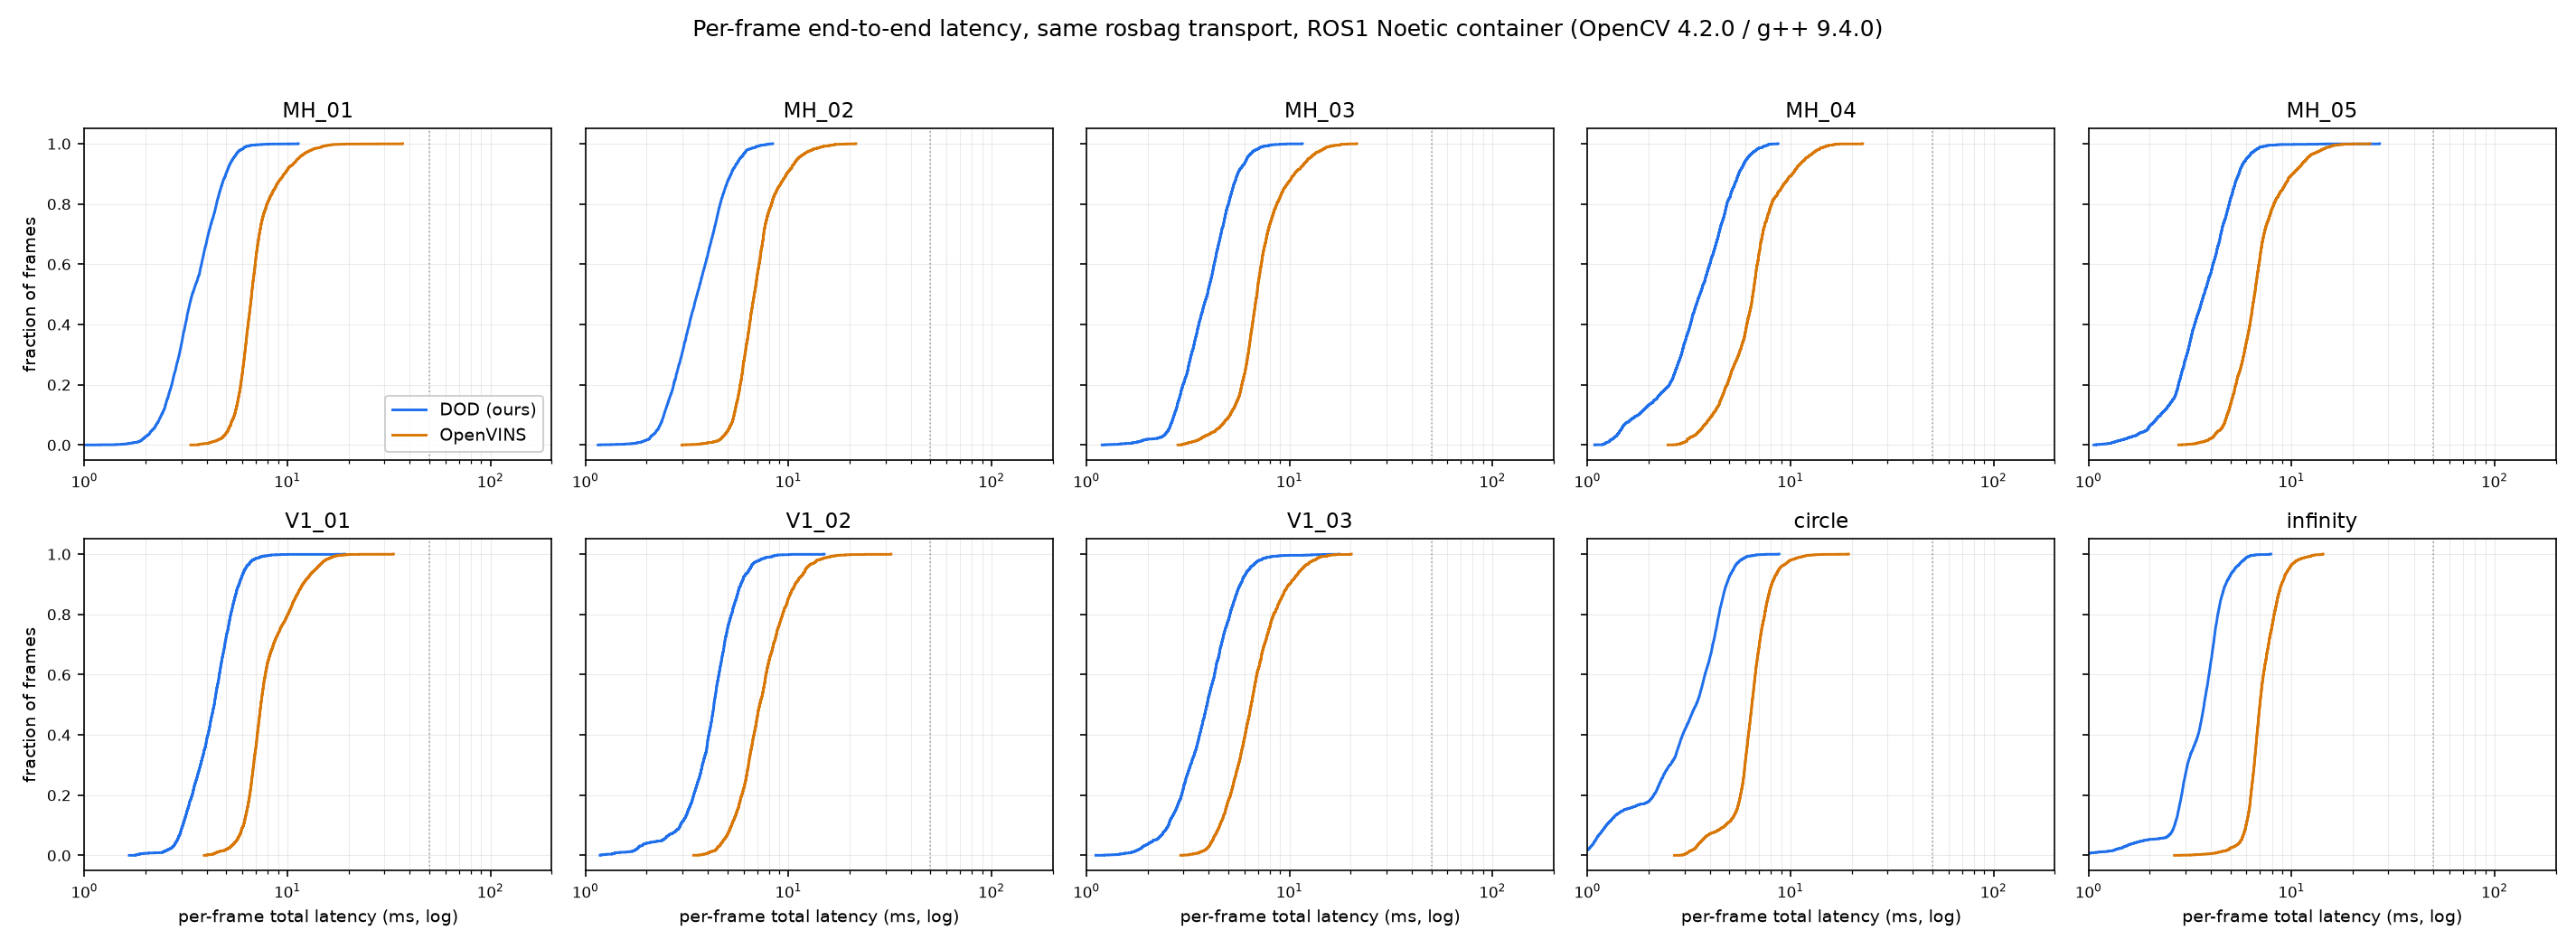
\includegraphics[width=\columnwidth]{figs/latency_cdf.png}
\caption{Per-frame latency CDFs on x86, both estimators, all ten sequences
(log scale; dotted line: the 50\,ms EuRoC 20\,Hz frame budget).}
\label{fig:cdf}
\end{figure}

The 99th-percentile ratio (1.64--2.05$\times$) exceeds the median ratio
(1.63--1.85$\times$) on 8 of 10 sequences: the tail is where the
data-oriented layout pulls further ahead, not behind. Worst observed frames
are 8.3--18.4\,ms for the reimplementation against 19.8--54.8\,ms for
OpenVINS, whose single worst frame (KAIST circle, 54.8\,ms) exceeds the
16\,Hz frame budget of that dataset. This is the paper's strongest single
latency number, and it is measured, not argued.

\subsection{Per-optimization ablation}

\begin{table*}[t]
\caption{Individually measured optimizations. Every row: all ten ATEs bit-identical before and after.}
\label{tab:ablation}
\centering
\begin{tabular}{cll}
\toprule
\# & Change & Effect \\
\midrule
1 & Feature DB: separate key order from payload storage & 9{,}556 memcpy/frame $\rightarrow$ 0 \\
2 & Exact early-accept for the $\chi^2$ gate ($S \succeq \sigma^2 I$ bound) & MSCKF $\chi^2$: 0.273$\rightarrow$0.079\,ms \\
3 & Square-root-form EKF update (Sec.~\ref{sec:sqrtform}) & S+inv: 0.436$\rightarrow$0.263\,ms; K: 0.272$\rightarrow$0.160\,ms \\
4 & $M_a = PH^\top$ as one GEMM instead of per-block products & 0.668$\rightarrow$0.461\,ms \\
5 & \texttt{STATE\_COV\_CAPACITY} 512$\rightarrow$384 (matches true worst case, 341) & Cov update: 0.745$\rightarrow$0.506\,ms \\
6 & DHAT-guided allocation cuts (3 sites) & 1{,}322{,}658$\rightarrow$825{,}790 blocks \\
7 & Measurement compression + $\chi^2$ restructuring & MSCKF stage: 1.535$\rightarrow$1.000\,ms \\
8 & $M_a$/covariance-update restructuring (first pass) & Per-frame: 7.40$\rightarrow$5.43\,ms \\
\bottomrule
\end{tabular}
\end{table*}

Table~\ref{tab:ablation} reports each change's independently measured effect,
each verified against the full ten-sequence ATE gate before being accepted.
Three of these changes were adopted only after a plausible-sounding guess
about their cause was profiled and found wrong: an early hypothesis that the
MSCKF update stage was slow because it processes roughly twice as many
features per update as OpenVINS was tested by capping the reimplementation
at OpenVINS's own cap of 40 features --- this changed the MSCKF stage
by only 3\% (1.581\,ms~vs.\,1.538\,ms) and cost accuracy on 6 of 8 sequences,
and was reverted. A second hypothesis, that the $M_a$ accumulation loop was
slow because it was structured differently from OpenVINS's own loop, was
also wrong --- OpenVINS has the identical nested loop structure --- though
restructuring it was still worth 2.2$\times$ for a different, profiled
reason (row 4). We report both negative results because the pattern
recurred: on this codebase, plausible causal narratives about where time
goes have been wrong more often than they have been right, and every change
in Table~\ref{tab:ablation} was accepted only after a profile, not a guess.

\subsection{Relative pose error: locating the accuracy gap}
\label{sec:rpe}

\begin{table}[t]
\caption{Relative pose error, 1\,s window (m), alignment-free.}
\label{tab:rpe}
\centering
\begin{tabular}{lrr}
\toprule
Sequence & Ours & OpenVINS \\
\midrule
MH\_01 & 0.0407 & 0.0406 \\
MH\_02 & 0.0384 & 0.0371 \\
MH\_03 & \textbf{0.0853} & 0.0936 \\
MH\_04 & \textbf{0.0811} & 0.0913 \\
MH\_05 & 0.1066 & 0.1078 \\
V1\_01 & \textbf{0.0084} & 0.0123 \\
V1\_02 & \textbf{0.0093} & 0.0140 \\
V1\_03 & \textbf{0.0140} & 0.0222 \\
\bottomrule
\end{tabular}
\end{table}

Table~\ref{tab:ate}'s aggregate ATE does not, by itself, indicate which
component of the pipeline --- initialization or the filter's steady-state
drift rate --- is responsible for a given sequence's result. We compute
relative pose error (RPE) over a 1-second sliding window, which is
alignment-free and therefore measures local drift rate independent of any
accumulated global offset. Table~\ref{tab:rpe} shows the reimplementation's
steady-state drift rate is better than OpenVINS's on five of eight EuRoC
sequences, statistically equal on two (MH\_01, MH\_05), and worse on one
(MH\_02, by 3.5\%). The filter itself is not, in aggregate, the source of
the ATE gap in Table~\ref{tab:ate}.

Decomposing MH\_01 and MH\_02 by elapsed time confirms where the gap
actually is: on both sequences the reimplementation initializes 1.8--2.8\,s
\emph{earlier} than OpenVINS (MH\_01: 1.3\,s vs.\ 3.1\,s; MH\_02: 2.0\,s
vs.\ 4.8\,s) and starts from a measurably worse initial state --- RMSE over
the first 5\,s of MH\_02 is 0.2133\,m for the reimplementation against
0.1188\,m for OpenVINS, despite near-identical drift rates thereafter
(0.1938\,m vs.\ 0.1022\,m over seconds 5--10, still elevated but converging).
That early-window offset does not fully wash out over the sequence: MH\_02's
overall ATE gap (Table~\ref{tab:ate}) is attributable to this initialization
transient, not to a persistent difference in filter quality.

\subsection{Fixing what silent failure paths hid}

The measurement effort in Sections~\ref{sec:rpe}--\ref{sec:embedded}
surfaced four defects on the frame-input path that a purely accuracy-driven
evaluation would not have found, because none of them fired on the ten
sequences evaluated in Table~\ref{tab:ate} and none moved a single ATE
digit when fixed. An IMU ring buffer discarded the \emph{newest} sample
once full rather than the oldest, meaning a sequence whose initializer had
not fired within 10{,}000 samples ($\approx$50\,s at 200\,Hz) would freeze
holding a window that could never advance to meet incoming camera frames ---
a permanent, silent initialization failure with no counter to make it
visible. An IMU-window selection routine silently truncated at a
scratch-buffer capacity and returned success on the truncated result. A
propagation step's boolean failure return was discarded by its caller, so a
non-advancing timestamp (never observed in bag playback, reachable on a live
sensor feed) would still trigger a full filter update against an
unpropagated state. All three now count their own rejections
(\texttt{imu\_buffer\_evictions}, \texttt{imu\_window\_truncations},
\texttt{frame\_unpropagated\_drops}) and are exercised in the fix's own
verification: all ten ATEs remained bit-identical and every counter reads
zero on every benchmarked sequence, confirming these paths were genuinely
unreached rather than merely undetected. We report this as a methodological
point as much as an engineering one: an accuracy benchmark that only ever
exercises well-behaved input data will not find defects that only manifest
under input the benchmark does not produce.

\section{Embedded Results on Jetson Orin Nano and a Cross-Platform Defect}
\label{sec:embedded}

To test the design where memory layout is supposed to matter most, both
estimators were built and run on an NVIDIA Jetson Orin Nano Super (6-core
Cortex-A78AE, 8\,GB LPDDR5, JetPack~6 / L4T~R36.4). Both were compiled inside
an aarch64 Ubuntu~20.04 container with GCC~9.4.0 and OpenCV~4.2.0 --- the
\emph{identical toolchain} as the x86 container of Section~\ref{sec:setup} ---
so that the only variable between the two platforms' results is the
processor. All ten benchmark sequences were run on-device for both
estimators through the same direct-rosbag transport as x86, and every run
recorded per-frame timing and peak RSS exactly as on x86
(Section~\ref{sec:results}).

\begin{table}[t]
\caption{Per-frame pipeline latency on the Jetson Orin Nano Super
(tracking + estimation, excluding bag I/O; ms; same toolchain container on
both sides, only the ISA differs).}
\label{tab:aarch64-latency}
\centering
\begin{tabular}{lrrrr}
\toprule
 & \multicolumn{2}{c}{Ours} & \multicolumn{2}{c}{OpenVINS} \\
\cmidrule(lr){2-3}\cmidrule(lr){4-5}
Sequence & p50 & p99 & p50 & p99 \\
\midrule
MH\_01   & 27.3 & 51.4 & 43.9 & 73.3 \\
MH\_02   & 27.3 & 51.1 & 42.9 & 71.1 \\
MH\_03   & 30.1 & 58.6 & 39.0 & 72.5 \\
MH\_04   & 27.0 & 54.4 & 41.8 & 74.2 \\
MH\_05   & 28.9 & 53.9 & 38.2 & 68.2 \\
V1\_01   & 35.3 & 57.1 & 47.4 & 81.8 \\
V1\_02   & 33.0 & 63.4 & 42.4 & 70.5 \\
V1\_03   & 30.6 & 62.7 & 38.8 & 68.0 \\
circle   & 28.6 & 50.9 & 34.5 & 56.5 \\
infinite & 29.3 & 45.0 & 34.1 & 54.8 \\
\bottomrule
\end{tabular}
\end{table}

\textbf{Latency.} Table~\ref{tab:aarch64-latency} shows the reimplementation
is faster on all ten sequences at both the median (1.16--1.61$\times$) and
the 99th percentile (1.08--1.43$\times$). Two honest observations qualify
this. First, the margin is \emph{narrower} than on the desktop x86, where
the median advantage was 1.63--1.85$\times$: whatever the mechanism behind
the desktop tail advantage (Section~\ref{sec:results}), it does not grow on
the small core --- p99 improves by less than p50 on 8 of 10 sequences here.
Second, absolute latencies are large: at EuRoC's 20\,Hz rate (50\,ms budget)
OpenVINS's p99 exceeds the frame budget on every sequence, and the
reimplementation's does on nine of ten, by 1--13\,ms. Neither estimator is
comfortably real-time on this device at 20\,Hz as configured; the
reimplementation is the only one whose \emph{median} stays within budget on
all ten sequences, and its peak RSS is flat (184--199\,MB across all ten
sequences, against OpenVINS's 98--179\,MB variable). The bounded-memory
design's cost is visible here too: it pre-allocates that working set whether
or not a sequence needs it.

\begin{figure}[t]
\centering
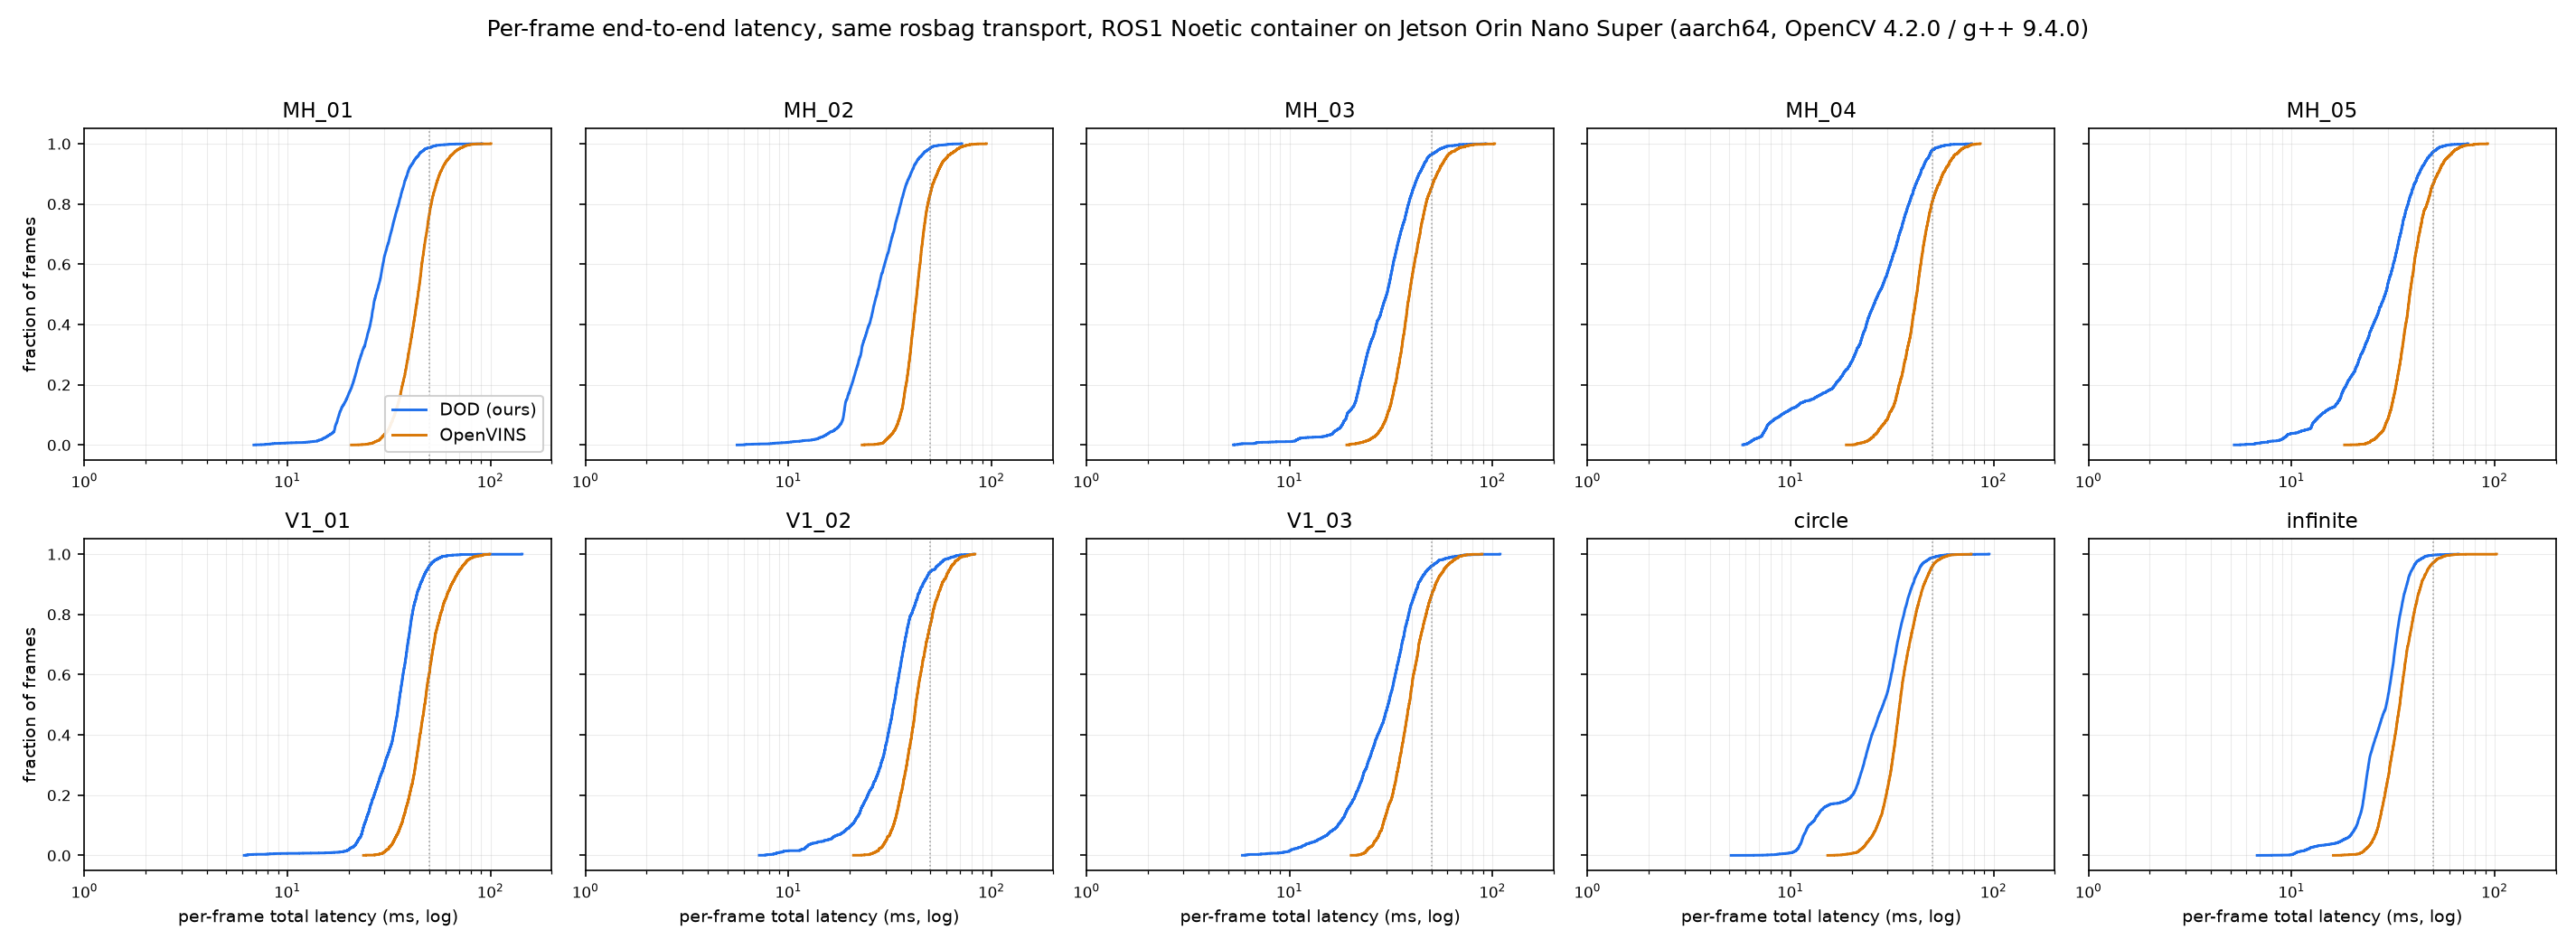
\includegraphics[width=\columnwidth]{figs/latency_cdf_aarch64.png}
\caption{Per-frame latency CDFs on the Orin Nano Super, both estimators,
all ten sequences (log scale; dotted line: the 50\,ms EuRoC 20\,Hz frame
budget). Direction matches x86 (Figure~\ref{fig:cdf}); the margin does
not.}
\label{fig:cdf-aarch64}
\end{figure}

\textbf{Accuracy on-device.} The reimplementation completed all ten sequences
without divergence. ATEs (the seven sequences for which the bag transport
yields ground truth on this device) sit in the same family as the x86
container's: MH\_01 0.1316 vs.\ 0.1293, MH\_02 0.1928 vs.\ 0.2080, MH\_03
0.2473 vs.\ 0.2343, MH\_04 0.3505 vs.\ 0.4267, MH\_05 0.3358 vs.\ 0.3285,
KAIST circle 0.0835 vs.\ 0.0374, infinity 0.0365 vs.\ 0.0261. Per
Section~\ref{sec:toolchain}'s lesson these are quoted as their own column,
not compared for parity: the KLT frontend's rounding behavior is part of the
platform, and KAIST circle --- the initialization-transient-sensitive
sequence of Section~\ref{sec:rpe} --- moves the most.

\textbf{What was not validated.} End-to-end wall-clock via
\texttt{hyperfine}, thermal/frequency state during measurement, and power
draw were not controlled or recorded; the per-frame latency figures above
are the embedded comparison this paper makes, and the CPU frequency governor
was left at its default on a passively cooled module, which a desktop
measurement does not have to worry about and this one does.

\textbf{The defect found.} A unit test covering a fallback path of the
dynamic initializer (Section~\ref{sec:featureless-init}'s primary
initializer's own fallback-of-a-fallback, reachable only when the
feature-less initializer itself fails) passed on x86 and failed on the
Jetson. The failure initially appeared to be a wrong-root selection in a
6$\times$6 companion-matrix eigenvalue solve --- the recovered gravity
direction printed as 171$^\circ$ from vertical, which looks like a sign
error. Instrumenting every candidate root on both platforms showed this was
a misdiagnosis: both platforms select the identical root by identical cost
criteria, and OpenVINS's own printed diagnostic for that same quantity reads
the same $\approx$171$^\circ$ on a passing x86 run, because that print was
never part of the root-selection or acceptance decision in the first place
(its associated threshold defaults to $10^9$ and is never overridden by any
shipped configuration). The actual divergence was a factor of three in a
downstream $|g|$-convergence residual (x86: 0.00034; aarch64: 0.00108),
straddling a hard-coded $10^{-3}$ absolute acceptance tolerance --- a
platform-dependent rounding difference through a QR-iteration eigenvalue
solve (SSE2 vs.\ NEON reduction order), not an algorithmic error. The
tolerance was widened to $3\times10^{-3}$, with the measured spread that
justifies the new value recorded alongside it; the fix was verified not to
move the eigenvalue selected, the $|g|$ residual's sign, or the ten
sequences' ATEs on x86 (this path is unreached on all ten). We report this
not because it is dramatic --- it affected a fallback of a fallback that
Table~\ref{tab:ate}'s benchmark never exercises --- but because it is
exactly the kind of defect a same-platform test suite cannot find, and one
we would not have found without attempting the embedded deployment this
section reports.

\section{Independent Evaluation on TUM VI}
\label{sec:tumvi}

Every result above was measured on datasets the pipeline's constants were
tuned against (EuRoC, KAIST), and our own altitude work showed that
inherited constants are the first thing that breaks on new data. As an
independent test, the pipeline was run on the TUM VI benchmark
\cite{schubert2018tumvi} with \emph{only its calibration adapted}: the
dataset's own pinhole-equi-512 Kalibr release was read verbatim into the
pipeline --- Kannala-Brandt~4 distortion through the existing equidistant
camera model, $T_{\text{cam\_imu}}$ in the convention the KAIST runner
already uses, and the BMI055 noise densities as shipped --- and every
estimator knob is the EuRoC placeholder, marked as such in the
configuration. Nothing in the pipeline was tuned on TUM VI. This is also
the first fisheye camera the pipeline has processed; EuRoC, KAIST, and the
embedded rig are all radtan-modelled.

\begin{table}[t]
\caption{TUM VI room sequences, ATE RMSE (m). Both estimators ran with the
dataset's own Kalibr calibration; OpenVINS received the same release as its
config, so the comparison is calibration-for-calibration.}
\label{tab:tumvi}
\centering
\begin{tabular}{lrr}
\toprule
Sequence & Ours & OpenVINS \\
\midrule
room1 & 0.0841 & \textbf{0.0693} \\
room2 & 0.0652 & \textbf{0.0542} \\
room3 & \textbf{0.0661} & 0.0871 \\
room4 & \textbf{0.0276} & 0.0359 \\
room5 & \textbf{0.0910} & 0.1011 \\
room6 & 0.0363 & \textbf{0.0327} \\
\midrule
Mean  & 0.0617 & 0.0634 \\
\bottomrule
\end{tabular}
\end{table}

\begin{figure*}[t]
\centering
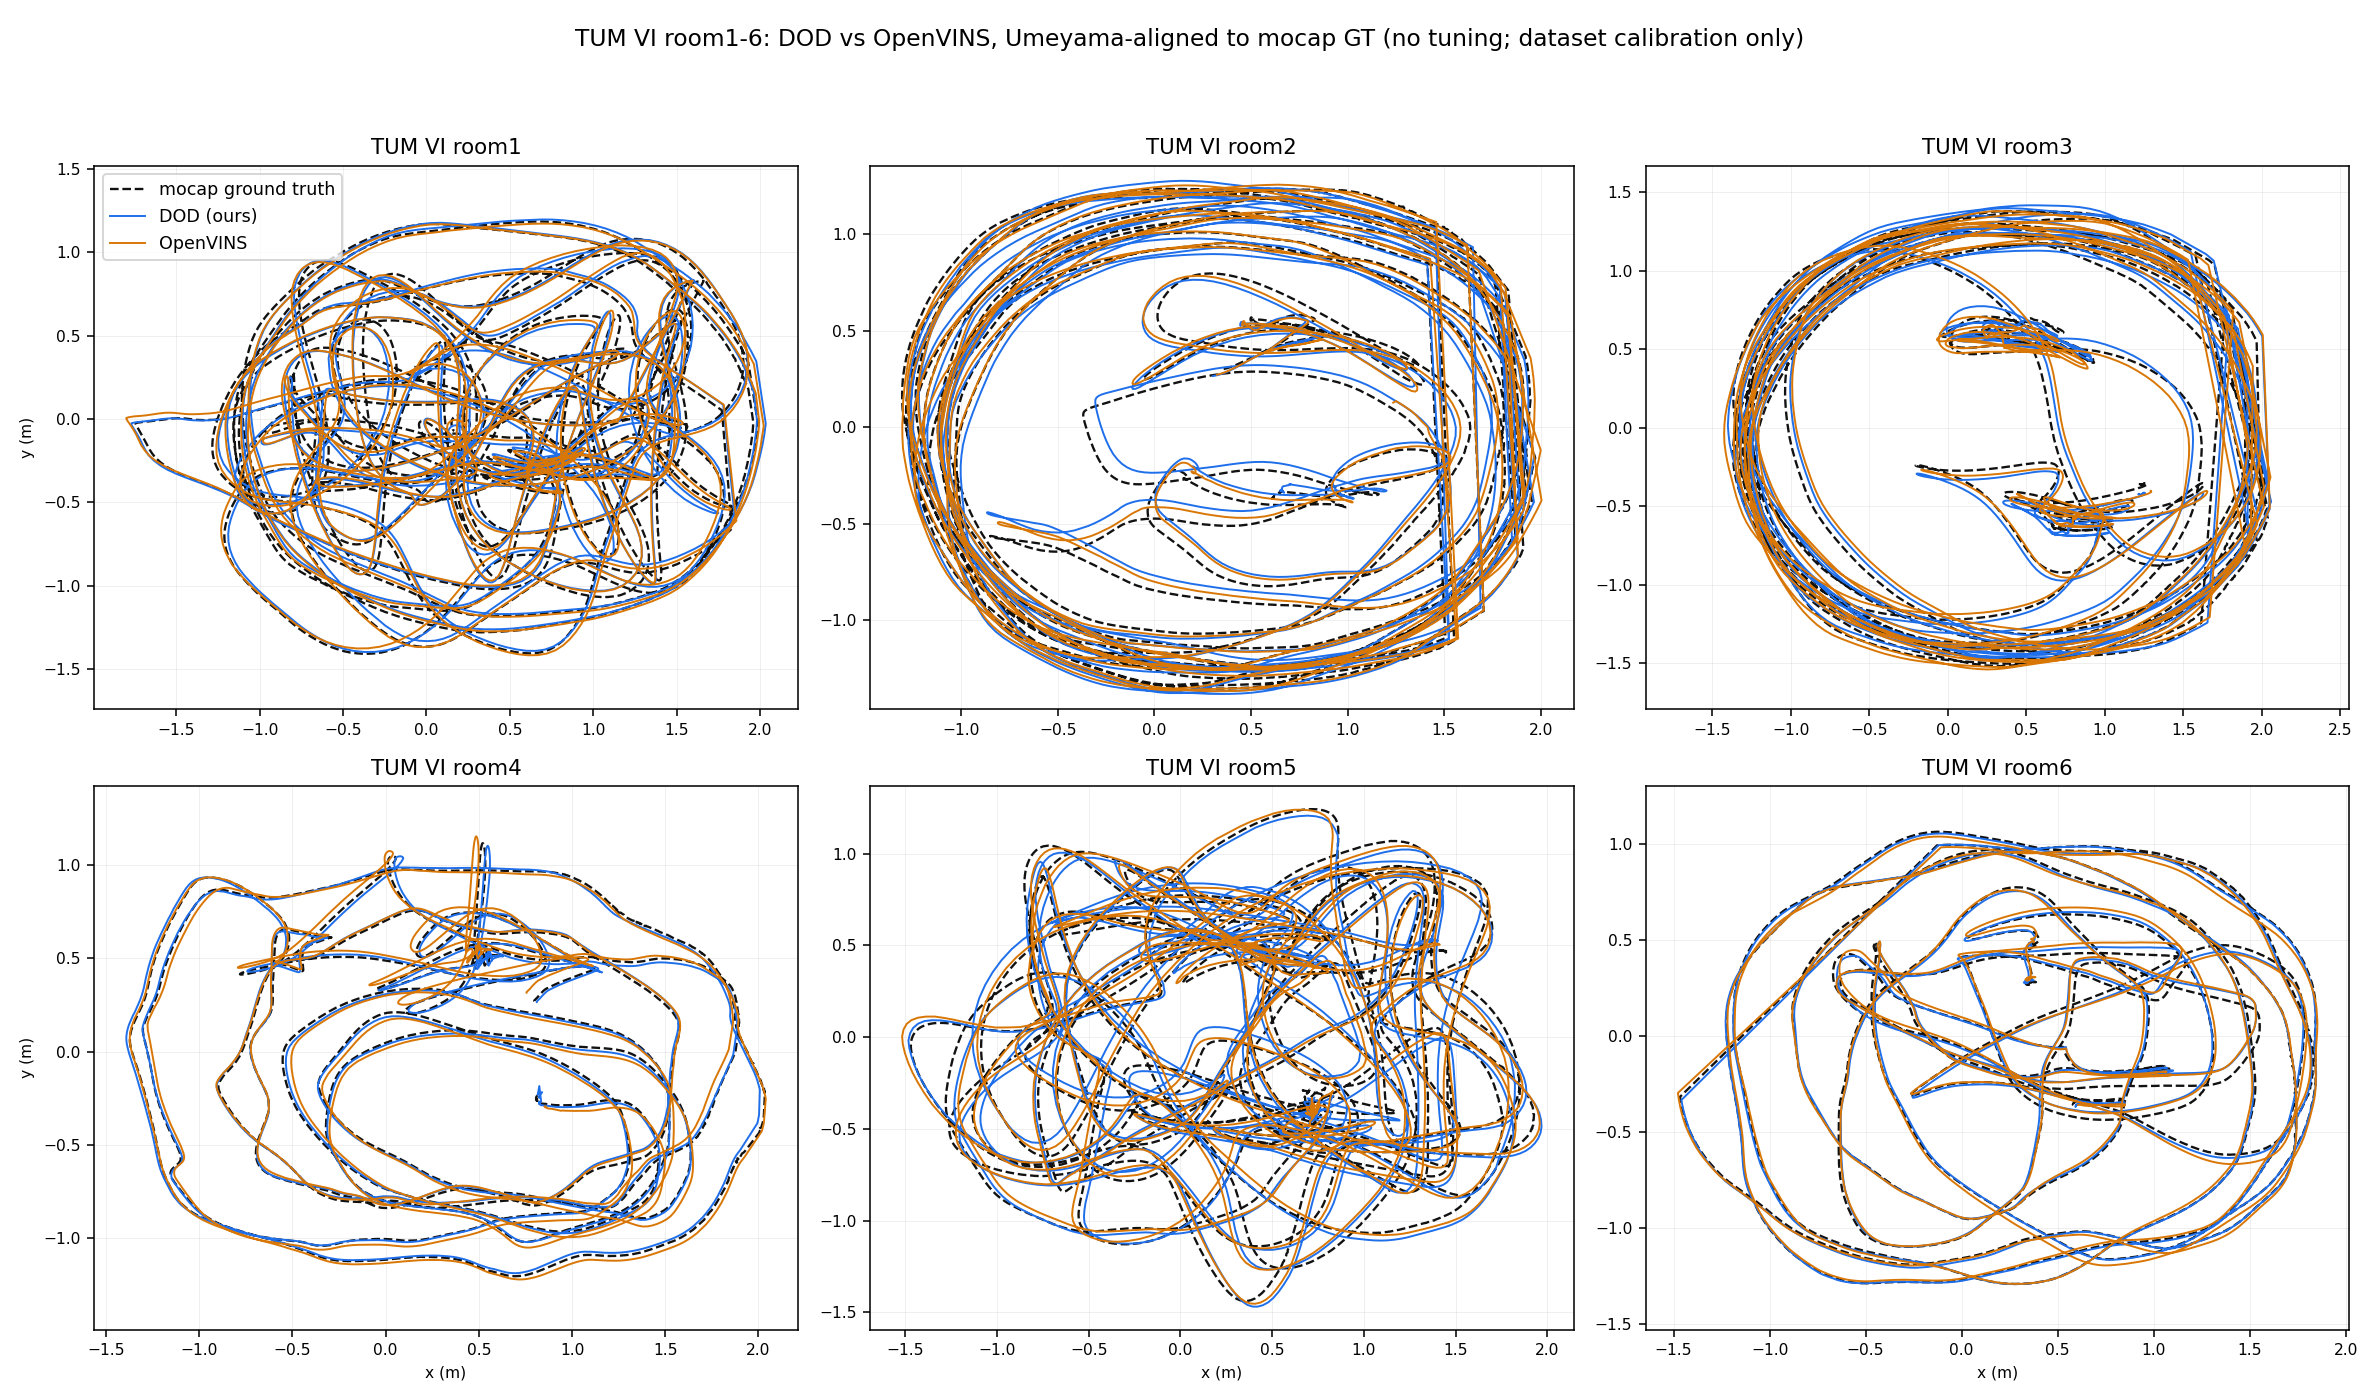
\includegraphics[width=\textwidth]{figs/tumvi_all_rooms.png}
\caption{TUM VI room1--6: both estimators Umeyama-aligned to the mocap
ground truth. All twelve runs (six per estimator) initialize and converge;
no sequence was tuned for.}
\label{fig:tumvi}
\end{figure*}

Table~\ref{tab:tumvi} and Figure~\ref{fig:tumvi} show the outcome: all six
room sequences initialize and converge with zero retuning, at accuracy
parity with OpenVINS (better on 3 of 6, mean 0.062\,m against 0.063\,m),
and with statistically indistinguishable drift --- the 1\,s-window relative
pose error (Section~\ref{sec:rpe}'s metric) is 0.0064--0.0101\,m for the
reimplementation against 0.0053--0.0101\,m for OpenVINS across the six
sequences. For a pipeline whose every constant was inherited from EuRoC
and KAIST, converging untuned on a third dataset family --- different
camera model, different IMU, different scene scale --- is the strongest
available evidence that the estimator is not overfit to its benchmarks.

\section{Limitations}
\label{sec:limitations}

\textbf{This is an implementation and measurement study, not a new
estimator.} Every filter equation in the primary pipeline is OpenVINS's;
the reimplementation's contribution is memory layout, and the honest framing
of every result in this paper follows from that: layout changes speed, not
accuracy, and Table~\ref{tab:ate} bears that out.

\textbf{Accuracy is parity, not superiority.} Better on 4 of 10 sequences,
mean ATE 0.156\,m against OpenVINS's 0.158\,m. A reader looking for a strict
accuracy win should not find one here; we report Table~\ref{tab:ate} in full
rather than a favorably selected subset.

\textbf{SchurVINS support is built but not benchmarked against the authors'
fork.} The reimplementation includes a data-oriented SchurVINS update path
(Section~\ref{sec:rules}'s constraints applied to \cite{fan2024schurvins}'s
algorithm), gated behind a runtime flag that defaults off, and verified to
run the full MH\_01 sequence to completion when enabled. No result in this
paper uses it: an earlier speed comparison
against the authors' own released \texttt{ov\_SchurVINS} fork was withdrawn
because the fork as released aborts on MH\_01 in our environment (in both
its serial and subscribe modes) and the build that produced the earlier
comparison no longer exists. We do not quote a number we cannot reproduce.

\textbf{Embedded comparison covers latency and memory, not the wall.}
Section~\ref{sec:embedded} reports both estimators on all ten sequences on
the Orin Nano with per-frame timing and peak RSS, but end-to-end wall-clock
under \texttt{hyperfine}, thermal state, and CPU frequency governor behavior
were not controlled or recorded; on a passively cooled module these can move
both sides. The allocation profile (DHAT) is x86-only.

\textbf{The TUM VI evaluation is x86-only and deliberately untuned.}
Section~\ref{sec:tumvi} runs on the desktop toolchain; repeating it on the
Orin Nano is future work. No estimator knob was swept on TUM VI --- that is
the design of the test, and it means the numbers there are the untuned
configuration's, not the pipeline's best.

\textbf{Monocular operation is not supported.} The tracker frontend requires
exactly two cameras; a single-camera front end would need new tracking code
(the estimator core already parameterizes camera count and would not
require changes) and has not been attempted.

\textbf{KAIST initialization latency was investigated and the obvious fix
rejected on evidence, not assumed away.} On KAIST~circle, the primary
initializer requires an accelerometer-variance jerk that does not occur
until 25.4\,s into the sequence (OpenVINS initializes at 3.7\,s via a
different trigger: its own KAIST configuration enables its zero-velocity
update at start, which changes which initializer branch it takes).
Reconfiguring the reimplementation to match --- initializing on the first
stationary window instead of waiting for a jerk --- was implemented,
measured, and found to produce a \emph{worse} trajectory (comparing only the
time window both configurations cover, to rule out a scoring artifact:
0.0464\,m vs.\ the shipped 0.0375\,m on circle, 0.0363\,m vs.\ 0.0261\,m on
infinity, both roughly 24\% worse), and was reverted. We report the negative
result rather than omit it: the correct fix requires replicating
OpenVINS's paired zero-velocity-update configuration for this specific
sequence, which is unimplemented, not merely untried.

\section{Conclusion}

Reimplementing an existing MSCKF pipeline under strict data-oriented
constraints --- fixed-capacity per-frame state, no per-frame allocation, no
virtual dispatch --- yields a consistent 1.76--2.10$\times$ end-to-end
wall-clock speedup over the reference OpenVINS implementation, measured
through an identical transport on ten public sequences, at accuracy parity
rather than accuracy superiority (mean ATE 0.156\,m against the reference's
0.158\,m, better on 4 of the 10 sequences and worse on 6). A finer-grained
relative-pose-error analysis shows the reimplementation's steady-state
filter quality is, if anything, slightly better than the reference on the
majority of EuRoC sequences, and that the aggregate accuracy gap is
concentrated in initialization-timing transients rather than in the
concentrated in initialization-timing transients rather than in the
estimator itself. Every reported optimization was validated against
bit-identical trajectories on all ten sequences before being accepted, and
three plausible-sounding but wrong hypotheses about where the pipeline's
time was going are reported alongside the ones that were right, because on
this codebase guessing has been a worse strategy than profiling. The
embedded deployment (Section~\ref{sec:embedded}) shows the advantage
transfers in direction but not in size --- faster on all ten sequences on
the Orin Nano, by a narrower margin than on desktop x86 --- and surfaced a
genuine cross-platform floating-point defect in an otherwise-unreached code
path, illustrating that even a same-architecture, bit-identical-trajectory
validation regime does not by itself certify cross-platform correctness.
Finally, an untuned run on the TUM VI benchmark
(Section~\ref{sec:tumvi}) --- a third dataset family and the first fisheye
camera model --- converges on all six room sequences at parity with
OpenVINS, evidence that the estimator is not overfit to the datasets its
constants were tuned on.
Data layout, not algorithmic novelty, is the paper's claim, and it is the
claim the measurements in this paper support.

\bibliographystyle{IEEEtran}
\begin{thebibliography}{10}

\bibitem{geneva2020openvins}
P.~Geneva, K.~Eckenhoff, W.~Lee, Y.~Yang, and G.~Huang,
``OpenVINS: A Research Platform for Visual-Inertial Estimation,''
\emph{Proc. IEEE Int. Conf. Robotics and Automation (ICRA)}, Paris, France, 2020.

\bibitem{mourikis2007msckf}
A.~I.~Mourikis and S.~I.~Roumeliotis,
``A Multi-State Constraint Kalman Filter for Vision-Aided Inertial Navigation,''
\emph{Proc. IEEE Int. Conf. Robotics and Automation (ICRA)}, Rome, Italy, 2007, pp. 3565--3572.

\bibitem{fan2024schurvins}
Y.~Fan, T.~Zhao, and G.~Wang,
``SchurVINS: Schur Complement-Based Lightweight Visual Inertial Navigation System,''
\emph{Proc. IEEE/CVF Conf. Computer Vision and Pattern Recognition (CVPR)}, 2024. arXiv:2312.01616.

\bibitem{peng2025sqrtvins}
C.~Peng \emph{et al.},
``sqrtVINS: Square-Root Filtering for Visual-Inertial Navigation Systems,''
\emph{IEEE Trans. Robotics (T-RO)}, 2025.

\bibitem{kottas2013hover}
D.~G.~Kottas, K.~J.~Wu, and S.~I.~Roumeliotis,
``Detecting and Dealing with Hovering Maneuvers in Vision-Aided Inertial Navigation Systems,''
\emph{Proc. IEEE/RSJ Int. Conf. Intelligent Robots and Systems (IROS)}, Tokyo, Japan, 2013, pp. 3172--3179.

\bibitem{fabian2018dod}
R.~Fabian,
\emph{Data-Oriented Design}, self-published, 2018.
\url{https://www.dataorienteddesign.com/dodmain/}

\bibitem{schubert2018tumvi}
D.~Schubert, T.~Goll, N.~Demmel, V.~Usenko, J.~St{\"u}ckler, and D.~Cremers,
``The TUM VI Benchmark for Evaluating Visual-Inertial Odometry,''
\emph{Proc. IEEE/RSJ Int. Conf. Intelligent Robots and Systems (IROS)}, Madrid, Spain, 2018.

\end{thebibliography}

\end{document}
